\section{Result}
\label{sec:analysis:result}


This sections presents results of the measurements of the branching
fractions using the two methods described earlier.  The values of the
branching fractions measured using the two approaches are shown in
Table~\ref{tab:results} and Figure~\ref{fig:wbr_result_1D}.  These plots
also show the current, best measured values of the W branching fractions
based on a combination of the measurements done by each of the LEP
experiments~\cite{Schael:2013ita}.  The measured values are strongly
correlated because of the construction of the model and because of the
constraint that the sum of branching fractions for leptonic and hadronic
decay modes be equal to one.  To demonstrate this, two dimensional
contours have been drawn and are shown in Figure~\ref{fig:contours_2D}.
Additionally, the covariance matrix for the branching fractions is show
in Figure~\ref{fig:correlation_matrix_POI}

One important distinction between the two measurements is that the MLE
method measures the branching fraction simultaneously in all final state
categories while the semi-analytic approach measures the branching fractions
separately in different trigger and b-tag categories and then combines
them using a $\chi^{2}$ fit.  

\begin{table}[htb!]
    \centering
    \setlength{\tabcolsep}{1.5em}
    \renewcommand{\arraystretch}{1.}
    \caption{Values of branching fractions determined in both
        analysis approaches and the PDG values.  Errors combine
        statistical and systematics uncertainties.
    \label{tab:results}}
    \begin{tabular}{l|ccc}
                           & counting              & shape                 & LEP \\
    \hline                                                                 
    w/o LU &&& \\
    \hline
    $W\rightarrow e\nu$    & $(11.15 \pm 0.27) \%$ & $(10.77 \pm 0.1) \%$  & $(10.71 \pm 0.16)$ \% \\
    $W\rightarrow \mu\nu$  & $(11.13 \pm 0.22) \%$ & $(10.91 \pm 0.08) \%$ & $(10.63 \pm 0.15)$ \% \\
    $W\rightarrow \tau\nu$ & $(10.63 \pm 0.65) \%$ & $(10.89 \pm 0.21) \%$ & $(11.38 \pm 0.21)$ \% \\
    $W\rightarrow h$       & $(67.08 \pm 0.72) \%$ & $(67.42 \pm 0.28) \%$ & $(-- \pm --)$ \% \\
    \hline
    w/ LU &&& \\
    \hline
    $W\rightarrow \ell\nu$ & $(-- \pm --)\%$       & $(10.87 \pm 0.07)\%$  & $(10.86 \pm 0.09)\%$  \\
    $W\rightarrow h$       & $(-- \pm --)\%$       & $(67.38 \pm 0.22)\%$  & $(67.41 \pm 0.27)\%$  \\
    \end{tabular}
\end{table}


\begin{table}[htb!]
    \centering
    \renewcommand{\arraystretch}{1.5}
    \caption{Correlation matrix of leptonic branching fractions.}
    \label{tab:results_corr}
    \resizebox{0.9\textwidth}{!}{
    \begin{tabular}{ccc}
        counting              & shape                 & LEP \\
      $\begin{bmatrix} 1 &+0.576 &-0.060 \\  +0.576 &1 &-0.265 \\ -0.265 &+0.714 &1 \end{bmatrix}$  
    & $\begin{bmatrix} 1 &+0.439 &+0.138 \\  +0.439 &1 &+0.190 \\ +0.138 &+0.190 &1 \end{bmatrix}$ 
    & $\begin{bmatrix} 1 &+0.136 &-0.201 \\  +0.136 &1 &-0.122 \\ -0.201 &-0.122 &1 \end{bmatrix}$ \\
    \end{tabular}}
\end{table}




            
\begin{figure}[htb!]
    \begin{center}
    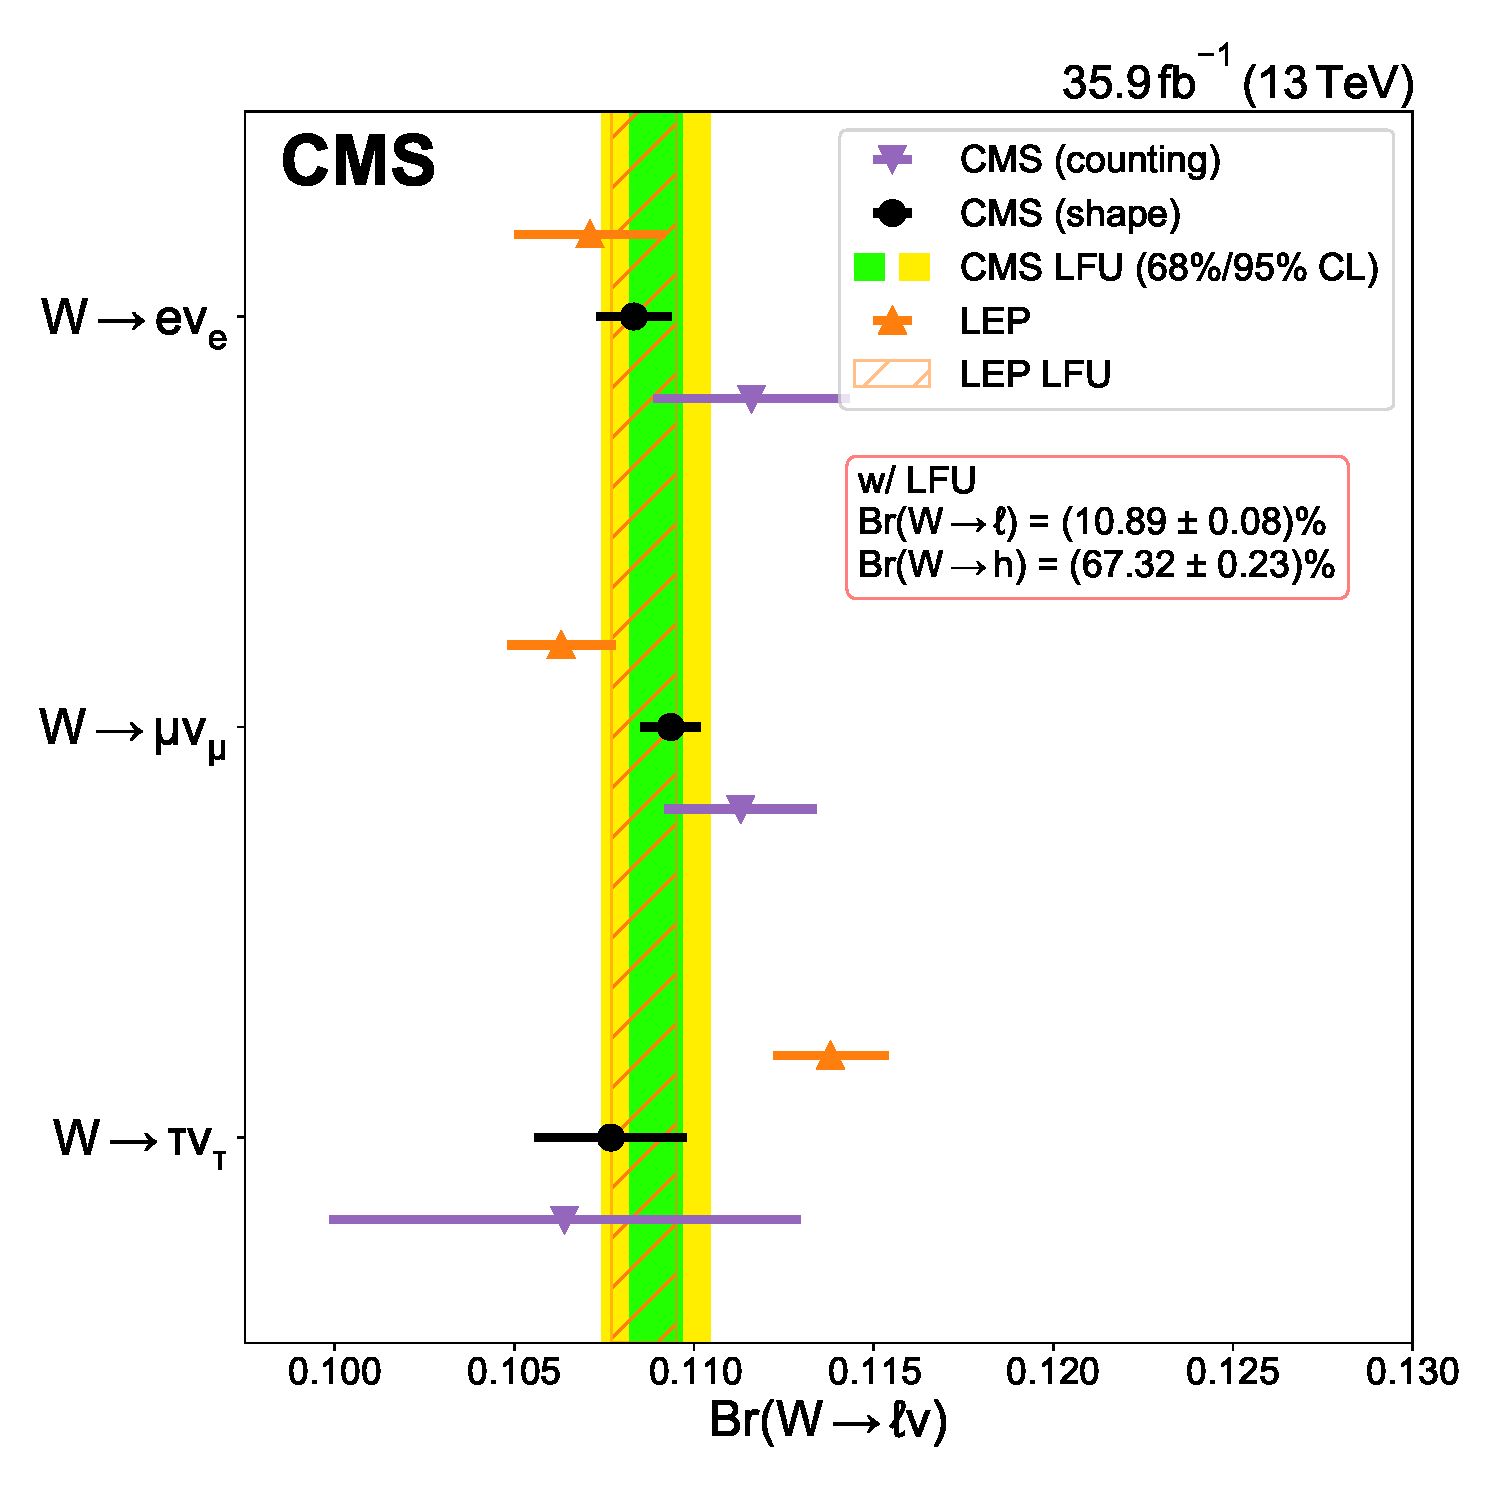
\includegraphics[width=0.95\textwidth]{chapters/Analysis/sectionResult/figures/unblinded_summary_plot.pdf}
    \caption{Summary of measured values of leptonic branching fractions.}
    \label{fig:wbr_result_1D}
    \end{center}
\end{figure}

\begin{figure}[htb!]
    \begin{center}
    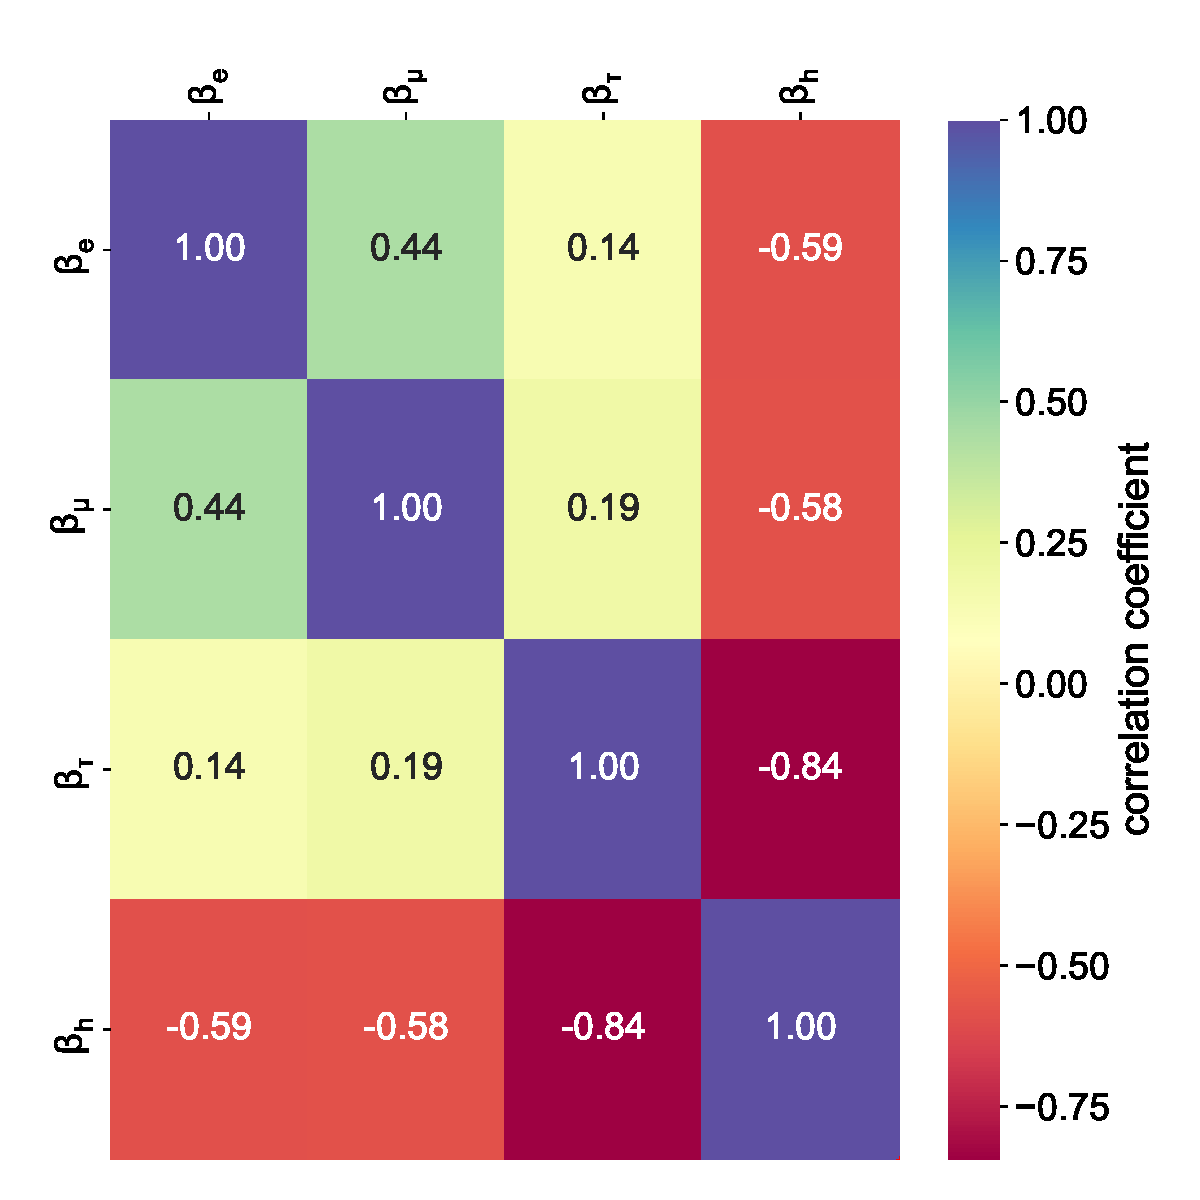
\includegraphics[width=0.5\textwidth]{chapters/Analysis/sectionResult/figures/correlation_matrix_POI_unblinded.pdf}
    \caption{Correlation matrix between each branching fraction component.}
    \label{fig:correlation_matrix_POI}
    \end{center}
\end{figure}

\begin{sidewaysfigure}[htb!]
    \begin{center}
    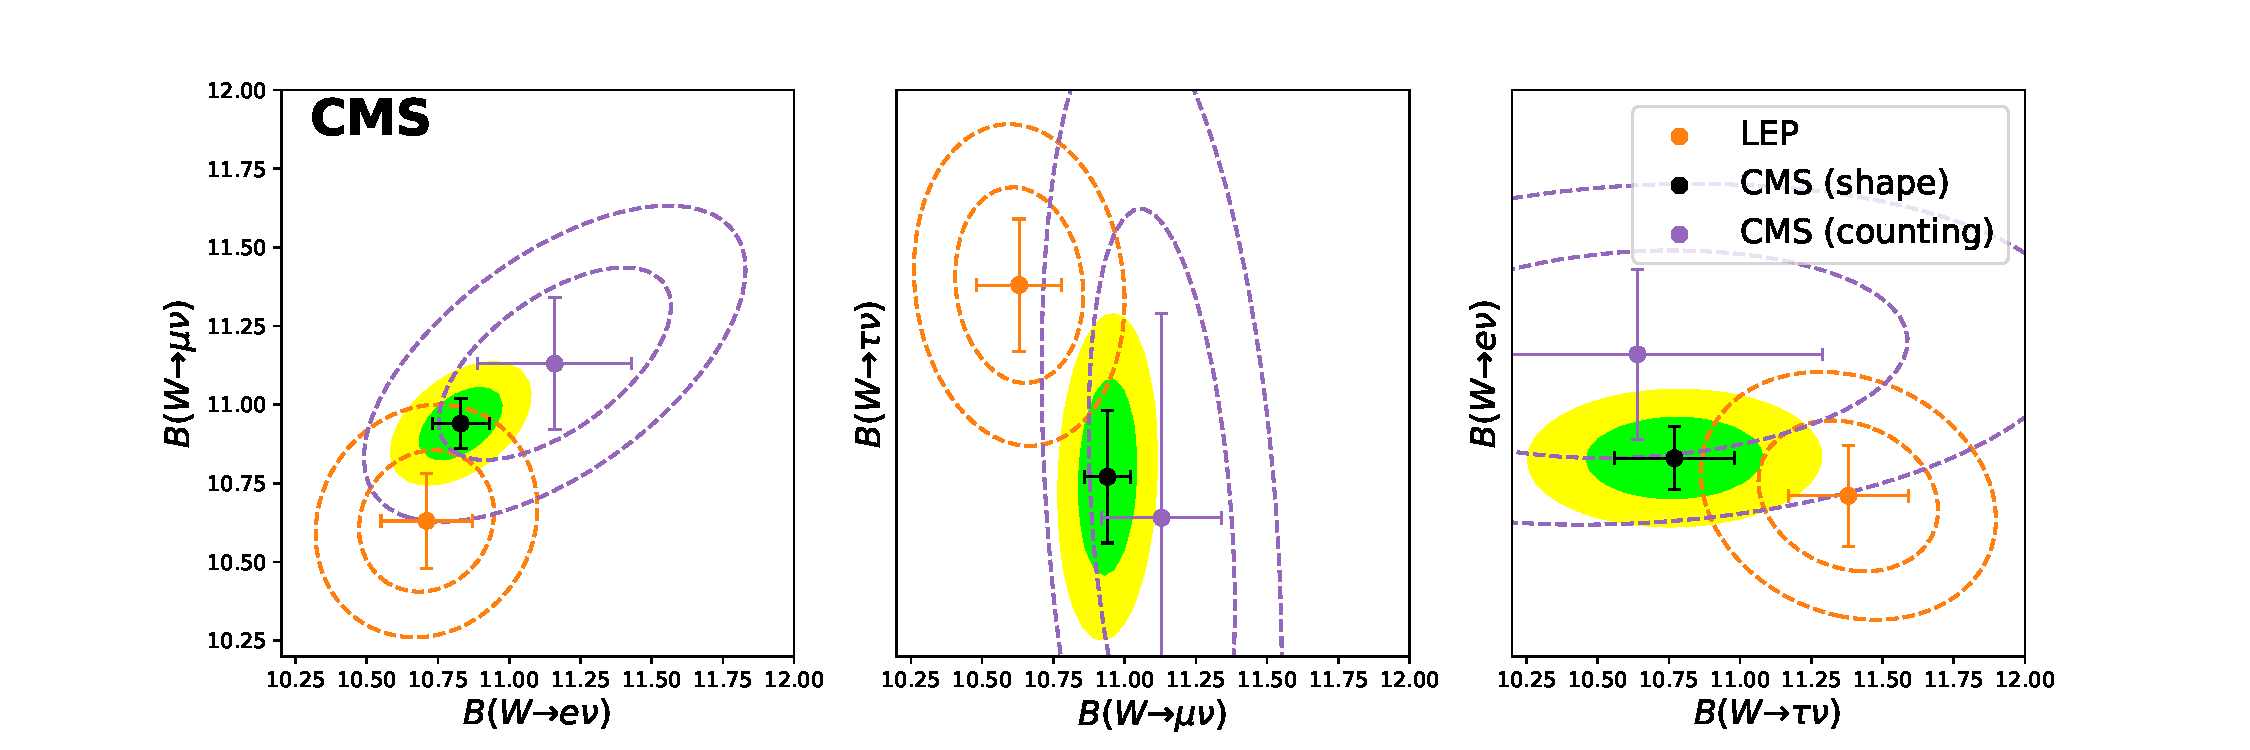
\includegraphics[width=0.95\textwidth]{chapters/Analysis/sectionResult/figures/result_contours_2d.pdf}
    \caption{Two dimensional comparisons of leptonic branching
    fractions.  For each pair shown in the panels, the branching
    fraction that is not shown has been marginalized over.  The dashed
    lines correspond to 68\% and 95\% contour levels for the resulting two
    dimensional Gaussian distribution.}
    \label{fig:contours_2D}
    \end{center}
\end{sidewaysfigure}



Having measured the branching fractions, it is of interest to calculate the
ratios between branching fractions and their pdfs to compare to values obtained
at other experiments where only ratios are measured.  To transform the
likelihood of the branching fractions to the likelihood for ratios, the following
integral transformation is evaluated\cite{10.2307/2334671},

\begin{equation}
    f(r) = \int_{-\infty}^{\infty} \left|b_{\ell}\right| g(r b_{\ell}, b_{\ell}) \,db_{\ell},
\end{equation}

where $r = b_{\ell'}/b_{\ell}$ and the PDF of the branching fractions
$g(b_{\ell_{1}}, \ell_{2})$ is a bivariate normal distribution with parameters
determined from the likelihood fit.  It is also possible to carry out the
transformation above for the two dimensional case so that ratios of all
elctrons and muons to taus can be compared as in Figure~\ref{fig:ratios_2D}.
Table~\ref{tab:ratios} shows comparisons between the ratios constructed from
the measurements described above, and those measured by LEP and ATLAS as well
as the SM expectation. 

\begin{figure}[htb!]
    \begin{center}
    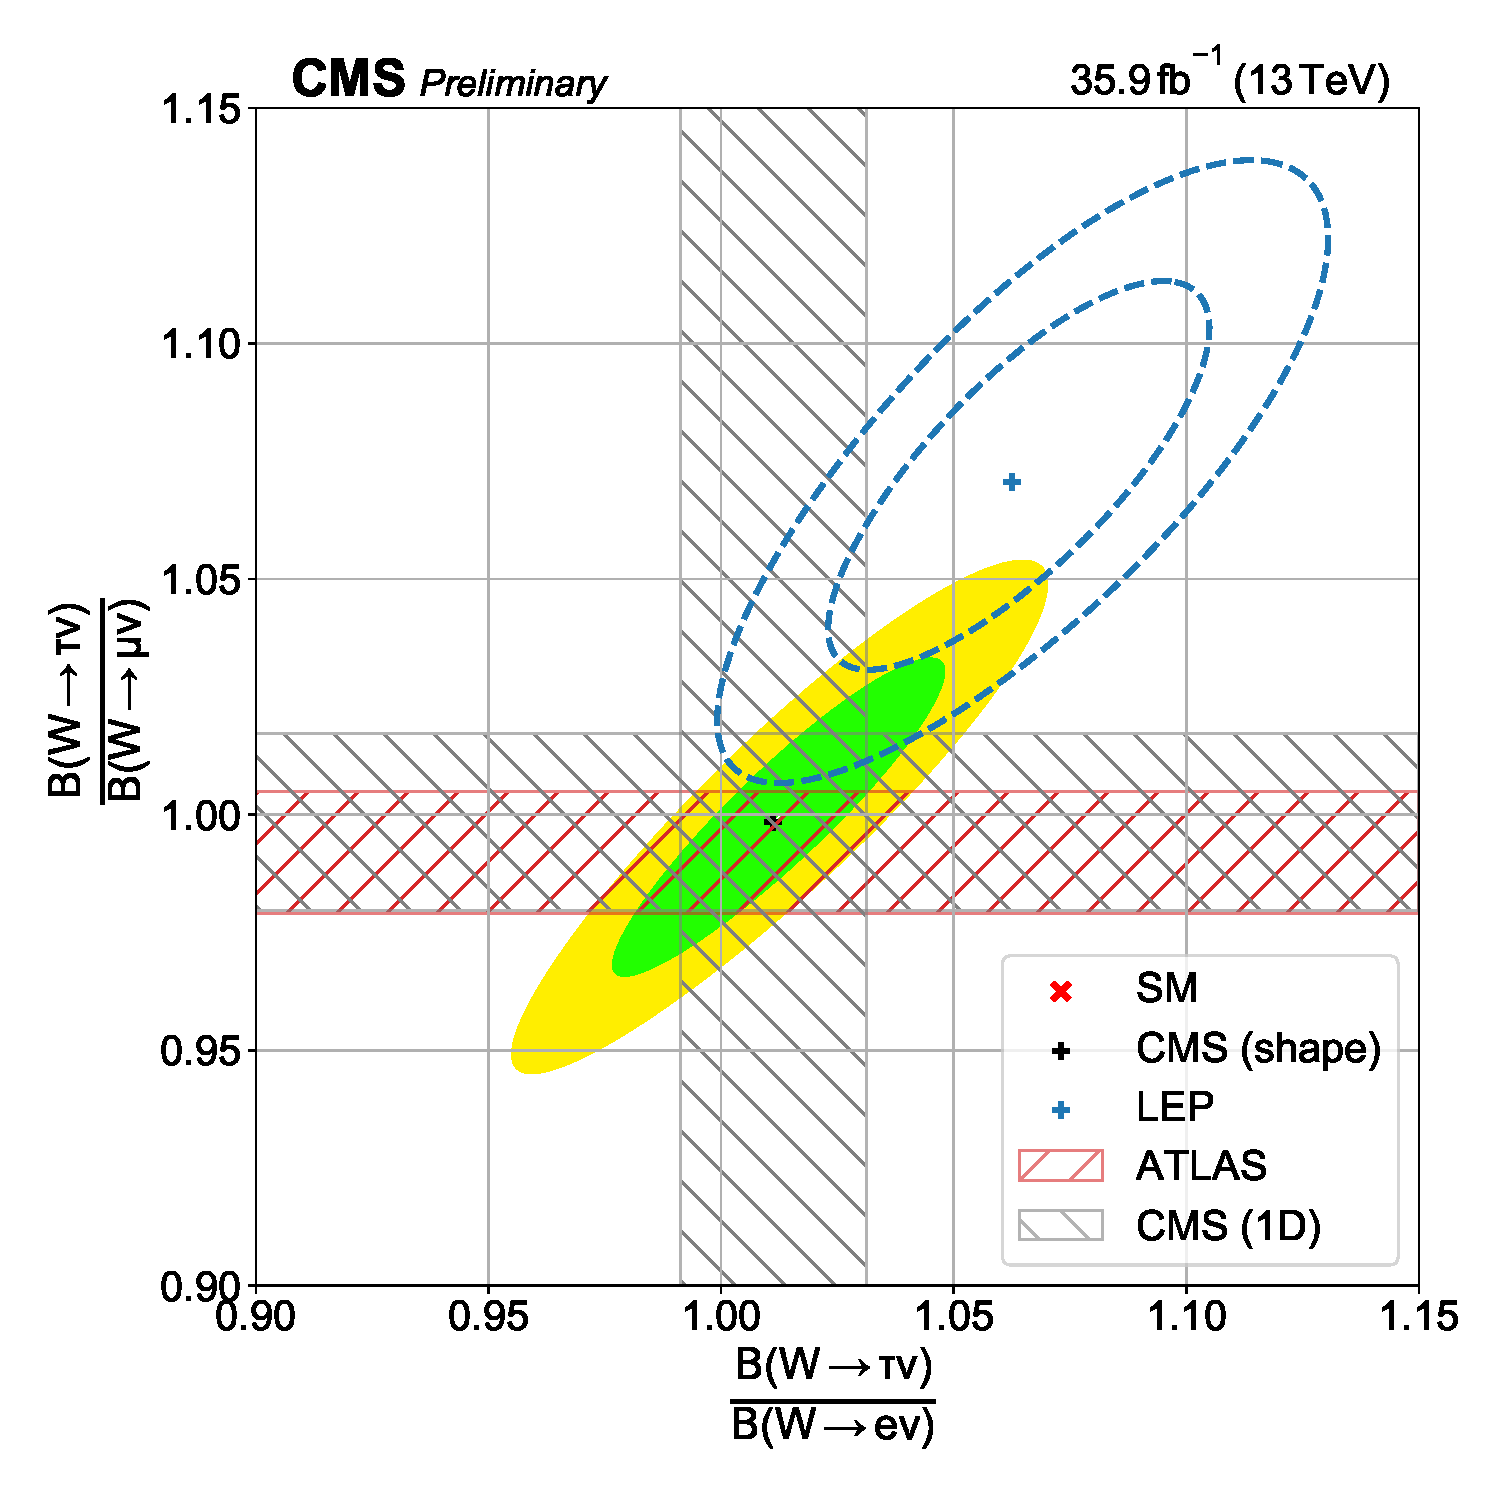
\includegraphics[width=0.95\textwidth]{chapters/Analysis/sectionResult/figures/result_contours_2d_ratio.pdf}
    \caption{Two dimensional distributions of the ratios $B(W\rightarrow
    \tau\nu)/B(W\rightarrow e\nu)$ vs $B(W\rightarrow \tau\nu)/B(W\rightarrow \mu\nu)$ 
    with comparisons of the CMS result to LEP and ATLAS measurements.}
    \label{fig:ratios_2D}
    \end{center}
\end{figure}

\begin{table}[htb!]
    \centering
    \topcaption{Ratios of branching fractions.
    \label{tab:ratios}}
    \begin{tabular}{l|ccc}
                                                                                               & CMS               & LEP               & ATLAS              \\
    \hline                                                                 
    $W\rightarrow \mu\nu / W\rightarrow e\nu$                                                  & $1.013 \pm 0.009$ & $0.993 \pm 0.019$ & --                 \\
    $W\rightarrow \tau\nu / W\rightarrow e\nu$                                                 & $1.011 \pm 0.020$ & $1.063 \pm 0.027$ & --                 \\
    $W\rightarrow \tau\nu / W\rightarrow \mu\nu$                                               & $0.998 \pm 0.019$ & $1.070 \pm 0.026$ & $0.992 \pm 0.013$  \\
    $2 W \rightarrow \tau\nu /(W\rightarrow e\nu + W\rightarrow \mu\nu)$                       & $0.98 \pm 0.27$   & $1.066 \pm 0.025$ & --                 \\
    \end{tabular}
\end{table}

The values of the leptonic branching fractions can also be used as a
check of the unitarity of the CKM matrix elements and calculating the
least well measured of the matrix elements, $\left|\rm V_{cs}\right|$.
To do both of these calculations, the following relation between the
leptonic branching fractions and CKM matrix elements is useful, 

\begin{equation}
    \frac{1}{\mathcal{B}(\mathrm{W} \rightarrow \ell\bar{\nu}_{\ell})} =
    3\left\{1 + \left[1 + \frac{\alpha_{S}(M^{2}_{\mathrm{W}})}{\pi}\right]
    \sum_{\substack{i = (\mathrm{u,c}), \\ j=(\mathrm{d, s,
    b})}}\left|\rm V_{ij}\right|^{2}\right\},
\end{equation}

where $\alpha_{S}(M^{2}_{\mathrm{W}})$ is the strong coupling constant
at the $\PW$ pole and $V_{ij}$ are the CKM matrix elements.  Solving for
$\sum_{ij}\left|V_{ij}\right|^{2}$ and using (these are the numbers used
for the LEP combination) a value of $\alpha_{S}(M^{2}_{\mathrm{W}}) =
0.119 \pm 0.002$ and sum over CKM matix elements squared excluding
$V_{cs}$ and $V_{tb}$ equal to $1.0544 \pm 0.0051$, the above expression
above can be used to calculate a value of $1.991 \pm 0.019$ is obtained.
Further solving for $\left|V_{cs}\right|$ yields a value of $0.968 \pm
0.010$.  The uncertainty on this quantity is almost entirely determined
by the experimental uncertainty of the leptonic branching fraction
measurment.






% \subsection{Branching Ratio}

% Test of lepton flavour universality (LFU) between electron and muons in 
% weak section has been performed to unprecedented precision
% in the past two decades. The tests have been carried out on both
% colliders and fix target experiments. Their results are shown
% in Table \ref{tbl:testlfuemu}. In general, the measurements
% branching ratios between electron and muon agree very well with 
% SM prediction.

% % \input{section6/tables/emutest.tex}

% In contract with agreement on LFU for $e$ and $\mu$ in weak section, LPU 
% regarding $\tau$ versus $e$ and $\mu$, as is discussed in Chapter 1, 
% is significantly challenged by 
% measurements from ALEPH, DELPHI, OPAL and L3 with LEP e+e- collision, 
% as well as Belle, Belle and LHCb with B meson decay.


% Therefore, we are interesed in the ratio of $Br (W\to \tau \nu)$ with respect to electron
% and muon channels,

% \begin{equation}
%     r = \frac{Br (W\to \tau \nu)}{Br (W\to l \nu)} , \text{ where } l=e,\mu
% \end{equation}

% based on the assumption that $Br (W\to \mu \nu) = Br( W\to e \nu )$, which
% is well justified by the previous precision test of LFU between $e$ and $\mu$ in weak section.
% This assumption is the same in Belle and BaBar measurements.

% The key to the success of Belle and BaBar measurements is that $tau$ are reconstructed
% by the same method as electron or muon, such that systematics regarding object
% reconstruction and selection are cancelled.
% Following this principle, we are measuring r in purely dilepton channels with muonic and electronic taus.
% Comparing with hadronic taus, this avoids the systematic uncertainty related to hadronic tau efficiency
% and misidentification.
% By using leptonic taus, systematics regarding lepton reconstruction 
% is canceled out to the first order, thus the precision of r is not limited systematically.

% The evolved dilepton channels are $\mu\mu$, $ee$ and $e\mu$ with $n_j \geq 2$ and $n_b = 1,2$,
% where $\mu\mu$, $ee$ also include $n_b = 0$ bin for Z background normalization purpose.
% r is obtained by simultaneous fit to the pT spectrum of the trailing lepton in $\mu\mu$,
% $ee$ and $e\mu$ channels. The methodology of this template fit is described in Section 5.3.
% The result is in Eqn \ref{eqn:fitr}.

% \begin{equation}
%     \boxed{
%     r = \frac{Br (W\to \tau \nu)}{Br (W\to l \nu)}
%     = 1.000 \times \big[1 \pm 2.72\% \text{ (stat)} \pm 1.44\% \text{ (syst)} \big]
%     }
%     \label{eqn:fitr}
% \end{equation}

% The correlation matrix of the fit is shown in Fig \ref{fig:covr}.

% The measurement of r using leptonic tau has small systematic uncertainty, thanks to the 
% cancellation of reconstruction efficiency. The precision of r is statistically limited, 
% which is expected to be improved when including 2017 data.


% The improvement of r precision when including more channels is shown in
% Fig \ref{fig:gain}. The gain of adding $e\mu$ and $\mu e$ channel is
% significant, while adding $l \tau$ and $l4j$ channel is small.


% \begin{figure}[p]
%     \centering
%     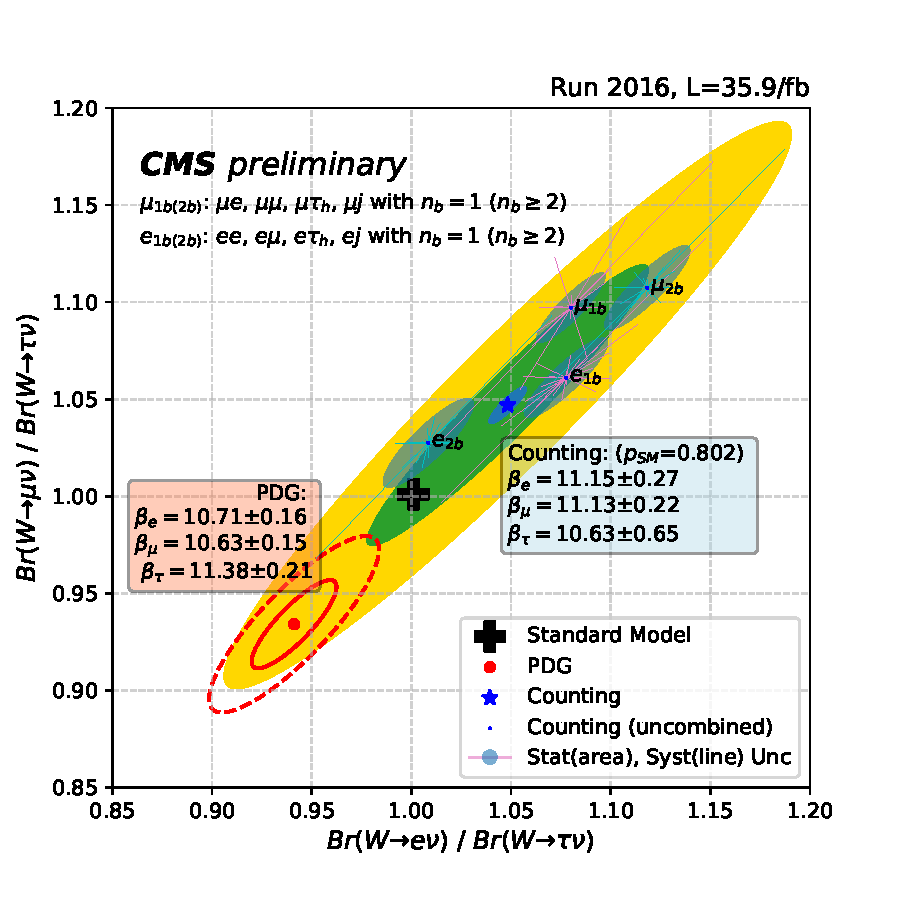
\includegraphics[width=14cm]{chapters/Analysis/sectionResult/figures/r2}
%     \caption{Fitting the pT spectrum of trailing lepton in $ee$, $\mu\mu$ and $e\mu$ channel.
%     The correlation matrix among r and systematic parameters.
%     }
%     \label{fig:covr}
% \end{figure}